%===============================================================================
% BIG DATA ANALYTICS PROJECT POSTER
% A3 Portrait Format - Diabetes Health Indicators Analysis
% Using tikzposter for professional academic poster design
%===============================================================================
\documentclass[a3paper, portrait, 25pt]{tikzposter}

%--- Packages ---
\usepackage[utf8]{inputenc}
\usepackage{graphicx}
\usepackage{booktabs}
\usepackage{multicol}
\usepackage{amsmath}
\usepackage{enumitem}
\usepackage{tikz}
\usepackage{helvet}  % Modern sans-serif font
\renewcommand{\familydefault}{\sfdefault}  % Use sans-serif as default
\usetikzlibrary{shapes.geometric, arrows.meta, positioning}

%===============================================================================
% COLOR THEME - Modern Professional Blue/Teal
%===============================================================================
\definecolor{PrimaryDark}{HTML}{1A365D}      % Dark navy blue
\definecolor{PrimaryLight}{HTML}{2B6CB0}     % Medium blue
\definecolor{AccentTeal}{HTML}{319795}       % Teal accent
\definecolor{AccentOrange}{HTML}{DD6B20}     % Orange for highlights
\definecolor{BackgroundLight}{HTML}{F7FAFC}  % Light gray background
\definecolor{TextDark}{HTML}{2D3748}         % Dark gray text

%--- Custom Color Theme ---
\definecolorstyle{DiabetesTheme}{
    \definecolor{colorOne}{named}{PrimaryDark}
    \definecolor{colorTwo}{named}{AccentTeal}
    \definecolor{colorThree}{named}{AccentOrange}
}{
    % Background Colors
    \colorlet{backgroundcolor}{BackgroundLight}
    \colorlet{framecolor}{PrimaryDark}
    % Title Colors
    \colorlet{titlefgcolor}{white}
    \colorlet{titlebgcolor}{PrimaryDark}
    % Block Colors
    \colorlet{blocktitlebgcolor}{PrimaryLight}
    \colorlet{blocktitlefgcolor}{white}
    \colorlet{blockbodybgcolor}{white}
    \colorlet{blockbodyfgcolor}{TextDark}
    % Innerblock Colors
    \colorlet{innerblocktitlebgcolor}{AccentTeal}
    \colorlet{innerblocktitlefgcolor}{white}
    \colorlet{innerblockbodybgcolor}{BackgroundLight}
    \colorlet{innerblockbodyfgcolor}{TextDark}
}

%--- Block Style ---
\defineblockstyle{RoundedBlock}{
    titlewidthscale=1, bodywidthscale=1, titleleft,
    titleoffsetx=0pt, titleoffsety=0pt, bodyoffsetx=0pt, bodyoffsety=0pt,
    bodyverticalshift=0pt, roundedcorners=15, linewidth=2pt,
    titleinnersep=8mm, bodyinnersep=10mm
}{
    \ifBlockHasTitle%
        \draw[rounded corners=\blockroundedcorners, fill=blocktitlebgcolor,
              draw=framecolor, line width=\blocklinewidth]
            (blocktitle.south west) rectangle (blocktitle.north east);
    \fi%
    \draw[rounded corners=\blockroundedcorners, fill=blockbodybgcolor,
          draw=framecolor, line width=\blocklinewidth]
        (blockbody.south west) rectangle (blockbody.north east);
}

%--- Apply Theme ---
\usetheme{Default}
\usecolorstyle{DiabetesTheme}
\useblockstyle{RoundedBlock}
\usetitlestyle{Filled}

%--- Title Setup ---
\title{\textbf{Diabetes Health Indicators Analysis}}

\author{
Ali Tarek Abdelmonim (21P0123) \quad
Andrea Aziz Fathy (23P0379) \quad
Fady Osama Mounir (23P0223)
Mohamed Mostafa Mamdouh (21P0244) \quad
Omar Baher Hussein (21P0315) \quad
Youssef Adel Albert (21P0258) \quad
}

\institute{Big Data Analytics Course -- Fall 2026}

%--- Graphics Path ---
\graphicspath{{outputs/plots/}}

%===============================================================================
\begin{document}
\maketitle[width=0.95\textwidth, titletoblockverticalspace=15mm]

%===============================================================================
% ROW 1: Problem Statement & Dataset Overview
%===============================================================================
\begin{columns}
    \column{0.5}
    \block{1. Problem Statement \& Objectives}{
        \textbf{\large Scientific Question:}
        \vspace{2.5mm}
        
        \textit{``Can self-reported lifestyle and demographic indicators stratify diabetes risk in population-level surveys---without invasive clinical tests?''}
        
        \vspace{2.5mm}
        \textbf{\large Project Objectives:}
        \begin{enumerate}[leftmargin=*, itemsep=2mm]
            \item \textbf{Explore} associations between modifiable behaviors and diabetes
            \item \textbf{Test} statistical hypotheses for key risk factors
            \item \textbf{Build} interpretable predictive models (ID3, Apriori)
            \item \textbf{Identify} top 3 actionable risk factors for public health
            \item \textbf{Evaluate} model performance with appropriate metrics
        \end{enumerate}
        
        \vspace{2.5mm}
        
\begin{tikzpicture}
            \node[draw=AccentTeal, fill=AccentTeal!10, rounded corners=8pt, 
                  text width=0.9\linewidth, align=center, inner sep=8pt] {
                \textbf{Impact:} Enable cost-effective population screening without requiring blood tests
            };
        \end{tikzpicture}
    }
    
    \column{0.5}
    \block{2. Dataset Overview}{
        \textbf{\large CDC BRFSS 2015 Survey Data}
        
        \vspace{2.5mm}
        \begin{center}
        \begin{tabular}{ll}
            \toprule
            \textbf{Attribute} & \textbf{Value} \\
            \midrule
            Total Records & 253,680 survey responses \\
            Features Used & 13 health indicators \\
            Target Classes & Healthy / Pre-diabetic / Diabetic \\
            Missing Values & None \\
            \bottomrule
        \end{tabular}
        \end{center}
        
        \vspace{2.5mm}
        \textbf{\large Key Features Analyzed:}
        \vspace{2mm}
        
        \begin{multicols}{2}
        \begin{itemize}[leftmargin=*, itemsep=1mm]
            \item \textbf{HighBP} -- Blood Pressure
            \item \textbf{HighChol} -- Cholesterol
            \item \textbf{BMI} -- Body Mass Index
            \item \textbf{PhysActivity} -- Exercise
            \item \textbf{Smoker} -- Smoking Status
            \item \textbf{Age} -- Age Group (1--13)
            \item \textbf{Education} -- Education Level
            \item \textbf{GenHlth} -- General Health
        \end{itemize}
        \end{multicols}
        
        \vspace{2.5mm}
        
\begin{tikzpicture}
            \node[draw=AccentOrange, fill=AccentOrange!10, rounded corners=8pt, 
                  text width=0.9\linewidth, align=center, inner sep=8pt] {
                \textbf{Class Distribution:} 80\% Healthy, 18\% Diabetic, 2\% Pre-diabetic
            };
        \end{tikzpicture}
    }
\end{columns}

%===============================================================================
% ROW 2: Key Visualizations
%===============================================================================
\block{3. Key Visualizations \& Analysis}{
    \begin{center}
    \begin{tikzpicture}
        % Image 1: BP vs Diabetes
        \node[anchor=north] (img1) at (0,0) {
            \includegraphics[width=0.22\linewidth]{1_bar_highbp_diabetes.png}
        };
        \node[below=2mm of img1, text width=0.22\linewidth, align=center, font=\small] {
            \textbf{High BP Effect}\\
            3x higher diabetic rate\\in hypertensive group
        };
        
        % Image 2: BMI Boxplot
        \node[anchor=north, right=8mm of img1] (img2) {
            \includegraphics[width=0.22\linewidth]{2_box_bmi_diabetes.png}
        };
        \node[below=2mm of img2, text width=0.22\linewidth, align=center, font=\small] {
            \textbf{BMI Gradient}\\
            Median: 27→30→31\\across groups
        };
        
        % Image 3: Age Trend
        \node[anchor=north, right=8mm of img2] (img3) {
            \includegraphics[width=0.22\linewidth]{4_line_age_diabetes.png}
        };
        \node[below=2mm of img3, text width=0.22\linewidth, align=center, font=\small] {
            \textbf{Age Trend}\\
            Prevalence: 0\%→25\%\\from age 18 to 80+
        };
        
        % Image 4: Correlation Heatmap
        \node[anchor=north, right=8mm of img3] (img4) {
            \includegraphics[width=0.22\linewidth]{8_heatmap_corr.png}
        };
        \node[below=2mm of img4, text width=0.22\linewidth, align=center, font=\small] {
            \textbf{Correlations}\\
            No multicollinearity\\detected ($|r|<0.5$)
        };
    \end{tikzpicture}
    \end{center}
}

%===============================================================================
% ROW 3: Analytical Methods
%===============================================================================
\begin{columns}
    \column{0.55}
    \block{4. Analytical Methods}{
        \vspace{2mm}
        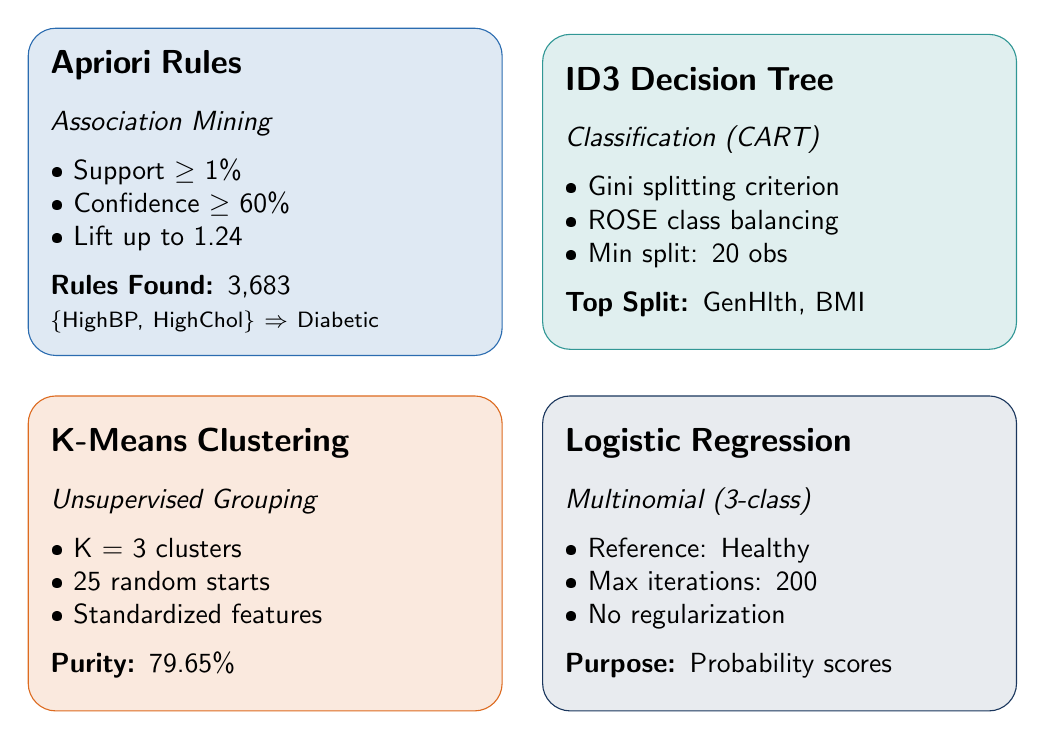
\begin{tikzpicture}
            % Method boxes
            \node[draw=PrimaryLight, fill=PrimaryLight!15, rounded corners=10pt,
                  text width=0.45\linewidth, minimum height=4cm, align=left, inner sep=8pt] 
                  (m1) at (0,0) {
                \textbf{\large Apriori Rules}\\[3mm]
                \textit{Association Mining}\\[2mm]
                • Support $\geq$ 1\%\\
                • Confidence $\geq$ 60\%\\
                • Lift up to 1.24\\[2mm]
                \textbf{Rules Found:} 3,683\\
                \footnotesize\{HighBP, HighChol\} $\Rightarrow$ Diabetic
            };
            
            \node[draw=AccentTeal, fill=AccentTeal!15, rounded corners=10pt,
                  text width=0.45\linewidth, minimum height=4cm, align=left, inner sep=8pt,
                  right=5mm of m1] (m2) {
                \textbf{\large ID3 Decision Tree}\\[3mm]
                \textit{Classification (CART)}\\[2mm]
                • Gini splitting criterion\\
                • ROSE class balancing\\
                • Min split: 20 obs\\[2mm]
                \textbf{Top Split:} GenHlth, BMI
            };
            
            \node[draw=AccentOrange, fill=AccentOrange!15, rounded corners=10pt,
                  text width=0.45\linewidth, minimum height=4cm, align=left, inner sep=8pt,
                  below=5mm of m1] (m3) {
                \textbf{\large K-Means Clustering}\\[3mm]
                \textit{Unsupervised Grouping}\\[2mm]
                • K = 3 clusters\\
                • 25 random starts\\
                • Standardized features\\[2mm]
                \textbf{Purity:} 79.65\%
            };
            
            \node[draw=PrimaryDark, fill=PrimaryDark!10, rounded corners=10pt,
                  text width=0.45\linewidth, minimum height=4cm, align=left, inner sep=8pt,
                  right=5mm of m3] (m4) {
                \textbf{\large Logistic Regression}\\[3mm]
                \textit{Multinomial (3-class)}\\[2mm]
                • Reference: Healthy\\
                • Max iterations: 200\\
                • No regularization\\[2mm]
                \textbf{Purpose:} Probability scores
            };
        \end{tikzpicture}
    }
    
    \column{0.45}
    \block{5. Results \& Key Insights}{
        \textbf{\large Model Performance:}
        \vspace{2.5mm}
        
        \begin{center}
        \begin{tabular}{lcc}
            \toprule
            \textbf{Model} & \textbf{Accuracy} & \textbf{AUC/Metric} \\
            \midrule
            Decision Tree & 69\% & AUC: 0.75 \\
            Logistic Reg. & 80\% & Macro-F1: 0.57 \\
            Apriori & -- & 3,683 rules \\
            K-Means & -- & Purity: 80\% \\
            \bottomrule
        \end{tabular}
        \end{center}
        
        \vspace{2.5mm}
        \textbf{\large Top 3 Risk Factors:}
        \vspace{2.5mm}
        
        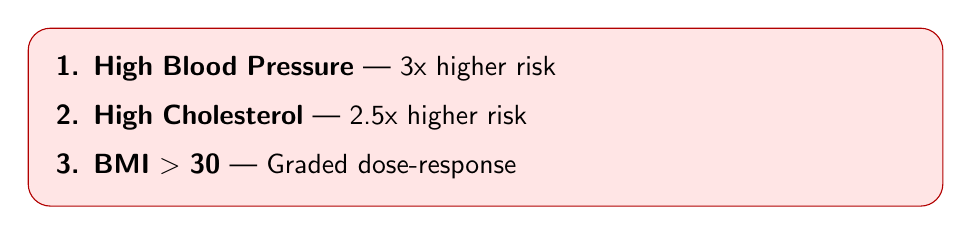
\begin{tikzpicture}
            \node[draw=red!70!black, fill=red!10, rounded corners=8pt,
                  text width=0.9\linewidth, align=left, inner sep=10pt] {
                \textbf{1. High Blood Pressure} --- 3x higher risk\\[2mm]
                \textbf{2. High Cholesterol} --- 2.5x higher risk\\[2mm]
                \textbf{3. BMI $>$ 30} --- Graded dose-response
            };
        \end{tikzpicture}
        
        \vspace{2.5mm}
        \textbf{\large Public Health Recommendations:}
        \begin{itemize}[leftmargin=*, itemsep=2mm]
            \item Target adults with HighBP + HighChol for screening
            \item Promote weight reduction (BMI $<$ 25)
            \item Increase physical activity programs
            \item Health literacy for underserved populations
        \end{itemize}

    \vspace{2.5mm}
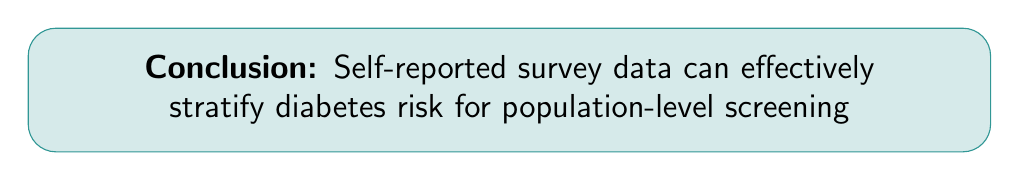
\begin{tikzpicture}
    \node[draw=AccentTeal, fill=AccentTeal!20, rounded corners=10pt,
          text width=0.95\linewidth, align=center, inner sep=10pt, font=\large] {
        \textbf{Conclusion:} Self-reported survey data can effectively\\
        stratify diabetes risk for population-level screening
    };
\end{tikzpicture}

    }
\end{columns}

%===============================================================================
% Footer with Hypothesis Summary
%===============================================================================
\block{Hypothesis Testing Summary (All p $<$ 0.001 --- All Significant)}{
    \begin{center}
    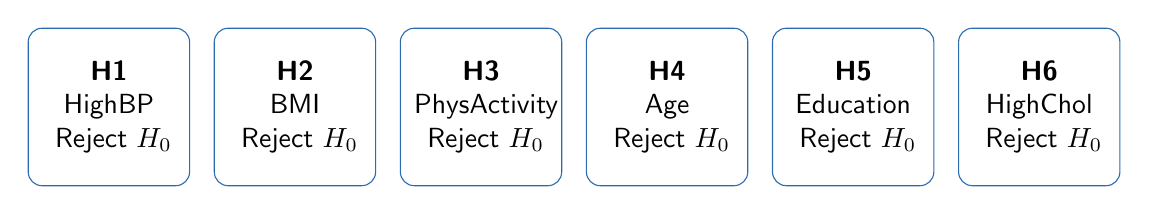
\begin{tikzpicture}
        % H1
        \node[draw=PrimaryLight, fill=white, rounded corners=5pt, 
              text width=0.14\linewidth, align=center, minimum height=2.0cm, inner sep=5pt]
              (h1) at (0,0) {\textbf{H1}\\HighBP\\$\checkmark$ Reject $H_0$};
        % H2
        \node[draw=PrimaryLight, fill=white, rounded corners=5pt, 
              text width=0.14\linewidth, align=center, minimum height=2.0cm, inner sep=5pt,
              right=3mm of h1] (h2) {\textbf{H2}\\BMI\\$\checkmark$ Reject $H_0$};
        % H3
        \node[draw=PrimaryLight, fill=white, rounded corners=5pt, 
              text width=0.14\linewidth, align=center, minimum height=2.0cm, inner sep=5pt,
              right=3mm of h2] (h3) {\textbf{H3}\\PhysActivity\\$\checkmark$ Reject $H_0$};
        % H4
        \node[draw=PrimaryLight, fill=white, rounded corners=5pt, 
              text width=0.14\linewidth, align=center, minimum height=2.0cm, inner sep=5pt,
              right=3mm of h3] (h4) {\textbf{H4}\\Age\\$\checkmark$ Reject $H_0$};
        % H5
        \node[draw=PrimaryLight, fill=white, rounded corners=5pt, 
              text width=0.14\linewidth, align=center, minimum height=2.0cm, inner sep=5pt,
              right=3mm of h4] (h5) {\textbf{H5}\\Education\\$\checkmark$ Reject $H_0$};
        % H6
        \node[draw=PrimaryLight, fill=white, rounded corners=5pt, 
              text width=0.14\linewidth, align=center, minimum height=2.0cm, inner sep=5pt,
              right=3mm of h5] (h6) {\textbf{H6}\\HighChol\\$\checkmark$ Reject $H_0$};
    \end{tikzpicture}
    \end{center}
}

\end{document}
